\section{Datasets}

The neural networks are trained and evaluated on images from 2 different datasets, KITTI\cite{kitti} and Lyft\cite{lyft2019}. Both datasets are preprocessed to remove frames where the camera is not moving. This is important because if there is no movement between frames then no depth information can be inferred during training when using monoscopic data. In the Kitti dataset the images from the left and right camera are treated as separate image sequences to yield more training data. The images are resized to $128\times 416$ pixels, and the intrinsic camera matrix is updated accordingly.

\subsection{Sequence datasets}

To train the networks used for depth and ego motion prediction the images from Kitti and Lyft at loaded in triplets of subsequent frames in a sequence.

The lidar data from Kitti and Lyft is converted to a sparse depth map, together with the ground truth ego motion. This data is only used during testing, not during training.
adjacent
\begin{figure}[H]
	\centering
	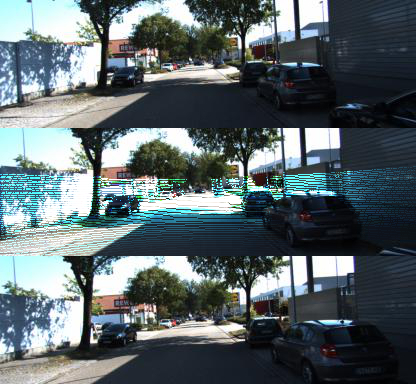
\includegraphics[width=0.5\textwidth]{sequencedataset}
	\caption{The dataloader loads 3 subsequent frames in a sequence. The figure shows from top to bottom 3 frames from Kitti, $I_{t-1}$, $I_t$, $I_{t+1}$ with the sparse depth map overlayed on frame $I_t$.}
	\label{fig:sequencedataset}
\end{figure}

Kitti contains 124 sequences, and Lyft contains 148 sequences. For each dataset the sequences are split, approximately 90\% is used for training and 10\% for testing.

\begin{table}[H]
	\centering
	\begin{tabular}{ |c|c|c|c|c| } 
		\hline
		&\multicolumn{2}{c|}{Sequences / Samples} \\ 
		\hline
		& Train & Test \\ 
		\hline
		Kitti & 110 / 16542 & 12 / 11349 \\ 
		\hline
		Lyft & 134 / 3759 & 14 / 1735 \\ 
		\hline
	\end{tabular}
	\caption{The training sequences are split into a training set and a testing set.}
	\label{table:datasets}
\end{table}

\subsection{Homographic adaptation dataset}

To train the network that predicts keypoints, images are read one by one from the Kitti or Lyft datasets. The image is fed trough two branches, in branch A the image is not modified, and in branch B the image is transformed by a random homography (Figure \ref{fig:unsuperpointloss}). The authors of UnsuperPoint refer to this technique as homographic adaptation.

How to generate the random homography used during training is not described in the UnsuperPoint paper, but is an important part of the method. The method used in this thesis generates random homographies from 5 parameters $\alpha_{rotation}$, $\alpha_{translation}$, $\alpha_{scale}$, $\alpha_{sheer}$ and $\alpha_{perspective}$. The parameters controls the maximum transformation for each aspect of an homography. The final homographgy is constructed from parts as follows.

\[
H = H_{affine} H_{sheer} H_{perspective}
\]

Assume $u_n \sim U(-1,1)$ are random uniform variables in the range -1 to 1.

\[
H_{affine} = 
\begin{pmatrix}
\cos(r)*s & -\sin(r) & t_x \\
\sin(r)& \cos(r)*s & t_y \\
0 & 0 & 1 \\
\end{pmatrix}
, \text{with}
\begin{cases}
r=u_1*\alpha_{rotation} \\
s=u_2*\alpha_{scale}+1 \\
t_x=u_3*\alpha_{translation} \\
t_y=u_4*\alpha_{translation} \\
\end{cases}
\]

\[
H_{sheer} = 
\begin{pmatrix}
1 & s & 0 \\
s & 1 & 0 \\
0 & 0 & 1 \\
\end{pmatrix}
, \text{with}
\ s=u_5*\alpha_{sheer} \\
\]

\[
H_{perspective} = 
\begin{pmatrix}
1 & 0 & 0 \\
0 & 1 & 0 \\
p & p & 1 \\
\end{pmatrix}
, \text{with}
\ p=u_6*\alpha_{perspective} \\
\]

The output from the network is used together with the random but known homography to formulate the loss function.

TODO: Illustration of training data for consensus maximization
